\chapter{Introduction}
Large pelagic fishes (LPF) including tunas, swordfish, and pelagic sharks, hold profound ecological
and economic importance globally. They are characterized by their highly migratory nature, and
their roles as apex predators. Their large-scale migrations are driven by the fact that food
resources and suitable breeding grounds are far apart from each other
\citep{fromentin_2005_tunareview,swordfish_migration,migration_lpf}. Through these migrations, LPF
form an important biological link between distant areas (trans-ocean migrations), and between
coastal and pelagic production \citep{linking_study}. As apex predators, they also strongly
influence the structure and function of ecosystems and intensive fishing can lead to cascading
top-down effects \citep{baum_worm_cascading,young15}. They also have a high social and global
importance for food security. Global catches of LPF, i.e., tuna and tuna-like species (mainly
Thunnini, Xiphiidae, and Istiophoridae), amounted to a record 8.3 million t reported landings in
2022, and tuna fisheries alone are worth 40 billion dollars annually
\citep{FAO2024,pew_tuna_value}.

\medskip

In the Mediterranean Sea \figref{fig:study_area}, bluefin tuna (BFT; \textit{Thunnus thynnus}),
albacore tuna (\textit{Thunnus alalunga}), and swordfish (SWO; \textit{Xiphias gladius}) are the
most important LPF \citep{fisheries_med_2000}. In 2023, these species alone accounted for
approximately 63\% of reported catches for all tuna and tuna-like species (in total around 60
thousand tonnes; \citealp{iccat_catches}). Apart from their economic importance, these three
species also form an important part of the culture and identity of numerous coastal communities in
the Mediterranean, as they have been exploited there since ancient times
\citep{cultural_social_addis,usai_22_culture,natale2005,andrews_ancient}. The bluefin tuna fishery
for example, is the oldest known industrial fishery in the world \citep{natale2012}.

\medskip

\begin{figure}[H]
	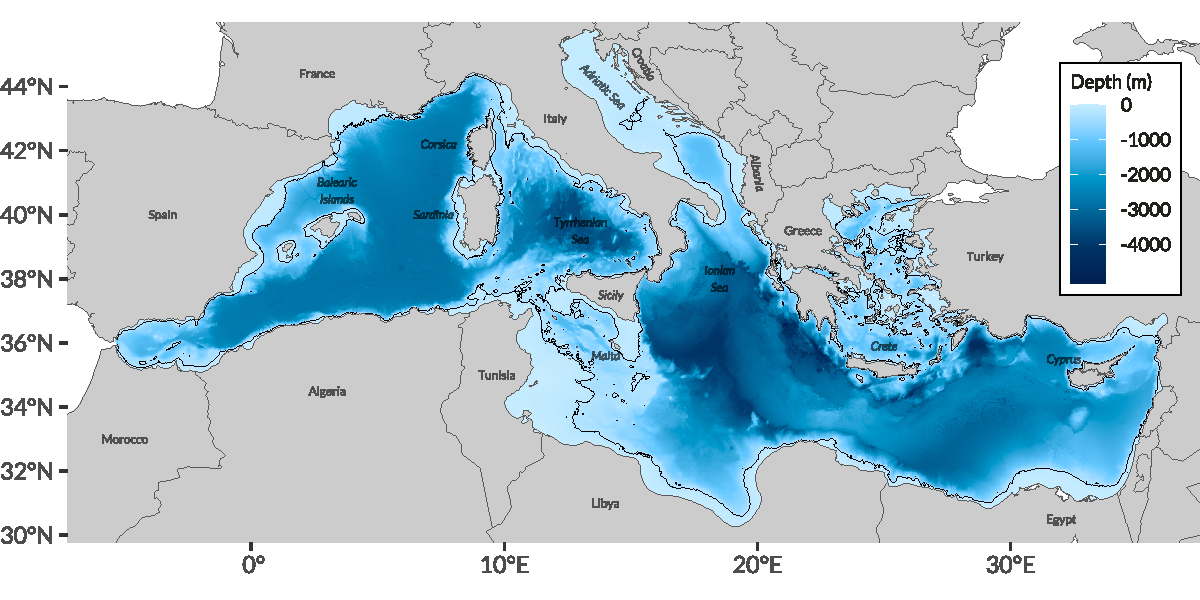
\includegraphics[width=1\linewidth, trim=0 0 0 0,clip]{Figures/plots/study_area_test.pdf}
	\caption{The Mediterranean Sea, study area for this analysis. The black line indicates the 200 m isobar.}
	\label{fig:study_area}
\end{figure}

\medskip

To sustainably manage these marine resources and the ecosystems they occur in, it is essential to
accurately estimate the location and intensity of fishing pressure
\citep{piet_fishing_indicators,russo_indicators,fishing_grounds_greece}. This information is
increasingly needed for efficient marine spatial planning, marine protected area designation,
conservation of target and non-target species, and ecosystem-based fisheries management
\citep{vespe_map_2016,henrique_effort_estimation,tidd_importance_effort,gerritsen2010,ais_mpa_designation,ais_bycatch,ais_bird_bycatch}.
Most fisheries management systems for example aim to regulate one or more of the following:
catches, gear type, fishing location, seasonality, and effort. To achieve this, information on
whom, when, where and how much fishing is occurring is necessary \citep{orofino_transparency}.

\medskip

To deal with the complex task of understanding the spatial distribution of fishing, traditionally,
mostly logbooks are used to monitor where and when a vessel is fishing \citep{HINTZEN201231}.
Compiling logbook data is the responsibility of each skipper and is mandatory for vessels fishing
in EU waters \citep{euregulation1993}. Information of catches is recorded daily at a spatial
resolution of 1° longitude and 0.5° latitude (size of ICES areas). Since the 2000s however, there
has been an increase in the usage of automatic monitoring tools. Since 2005, Vessel Monitoring
Systems (VMS) are mandatory for fishing vessels >15 m in the EU, to meet the increasing need for
fine-scale spatial and temporal information from commercial fleets for compliance with the
ecosystem approach to fisheries management \citep{ec2003regulation,gerritsen2010}. In the EU, VMS
usually have a ping rate between 1-2 hours, aiming at a compromise between appropriate resolution
and costs \citep{shepperson}. This data has however traditionally been confined to government
regulators and other fisheries authorities, limiting its usage, particularly in the case of
migratory species that travel between different countries' jurisdictions
\citep{orofino_transparency,confidentiality}. More recently, the usage of Automatic Identification
Systems (AIS) has emerged as a promising tool to monitor the spatio-temporal extent of fisheries
and for fisheries Monitoring, Control and Surveillance (MCS; \mbox{\citeauthor{zhang_ais_mcs},
	\citeyear{zhang_ais_mcs}}). Globally, AIS is compulsory for large vessels (over 300 tons), while in
the EU it is mandatory for fishing vessels $\ge$15m in length \citep{ec2011directive}. Originally
designed as a collision avoidance tool, it allows analysis at higher spatial and temporal
resolution due to the high ping rate of up to 2 seconds
\citep{taconet2019global,kontasvesselupdate}. There are however some handicaps that can limit the
coverage of this technology. This includes for example intentional turning-off, reception quality,
and difficulty of discerning individual messages in areas with very high vessel density
\citep{taconet2019global}. The increasing coverage and data availability however, enable the
analysis of more complex fisheries behaviours \citep{natale} and AIS data is also publicly
accessible, allowing for a fine-scale spatio-temporal assessment of fisheries between different
countries' jurisdictions.

\medskip

Most studies investigating fishing effort in the Mediterranean Sea have looked at the spatial
footprint of bottom trawlers as shown by \cite{ferra_trawlers_change} and
\cite{marsaglia_trawling}. However, monitoring the fisheries on LPF in this area will also provide
important information for their management. The International Commission for the Conservation of
Atlantic Tunas (ICCAT) is responsible for the sustainable management of LPF in the Mediterranean.
Spatio-temporal data on fishing effort are incorporated into stock assessments for bluefin tuna,
swordfish, and albacore tuna \citep{iccat_bft_summary,iccat_swo_summary,iccat_alb_summary}.
However, the data reported by contracting parties are often coarse in resolution (aggregated at 5°
x 5° or more rarely 1° x 1°) which limits the capacity to detect fine-scale fishing patterns.
Incorporating fishing pressure derived from AIS, could provide an alternative for cross-validation
of reported effort data and analysis on a finer spatial scale.

\medskip

Monitoring fisheries of LPF is also highly relevant in terms of climate change, of which the
effects have recently been proposed to be integrated in the species' management
\citep{iccat_climate_change}. For this, members of the ICCAT "\textit{Subcommittee of Ecosystems
	and Bycatch}" have created the "\textit{TunaMed Observatory}" with the aim to "\textit{identify and
	monitor the variability of environmental processes in the Mediterranean Sea that affects the
	ecology of large pelagic fishes - with special attention on tunas-, and to investigate the
	potential role of climate change on this variability}" \citep{tunamed}. As the spatial footprint of
fishing is closely linked to the distribution of target species, changes in the distribution of
fishing could thus be indicators of habitat change and climate-driven shifts in species range
\citep{fishing_climate_change_shifts}.

\medskip

One of the most important gear types used in the Mediterranean for the capture of LPF are drifting
longlines \citep{FAO2025Longlines,iccat_alb_summary,iccat_bft_summary,iccat_swo_summary}. This gear
type is however also associated with high levels of bycatch which includes species of sea turtles,
pelagic sharks, and seabirds \citep{bycatch_book}. Thus, demonstrating the utility of fine scale
fishing data for the conservation of non-target species for example through combining both species
distribution models with this data \citep{welch_overlap_ais_bycatch}. Apart from longlines, purse
seine nets are used in the Mediterranean mainly for the capture of BFT, targetting schools of these
fish during spawning. In the Mediterranean, this method is not associated to large amounts of
bycatch but can have big impacts on the targetted fish as it is extracting whole schools
\citep{bycatch_book,iccat_bft_summary}

\medskip

To address current gaps in the monitoring of large pelagic fisheries in the Mediterranean, this
thesis uses fine-scale data on fishing activities derived from AIS and provided by Global Fishing
Watch (GFW) to examine spatio-temporal patterns in fishing over the past decade (2015-2024). This
approach enables analysis of the whole Mediterranean Sea area, that would not be possible when
relying on other effort estimates like VMS and logbooks. The study focuses on the two main gear
types targeting LPF, namely drifting longlines and tuna purse seines, to determine
"\textit{hotspots}" of fishing activity (as an indicator of high risk areas for LPF), analyse
temporal trends, and determine differences in the spatio-temporal distribution pattern by both
fleets. More specifically, we aim to answer:
\begin{enumerate}
	\item Where and when is fishing activity for large pelagic species most intense and have spatial patterns
	      shifted between 2015 and 2024?
	\item What are the seasonal patterns of fishing activity by gear type and do temporal patterns differ
	      inter-annually?
	\item To what extent does AIS capture the full scope of fishing activity in the Mediterranean?
	\item What is the spatial relationship between fishing hours and environmental features such as distance
	      to port and depth?
\end{enumerate}